\documentclass[12pt]{article}
\usepackage[frenchb]{babel}
\usepackage{fontspec}
\usepackage{amsmath}
\usepackage{amsfonts}
\usepackage{amssymb}
\usepackage{graphicx}
%\usepackage[left=2cm,right=2cm,top=2cm,bottom=2cm]{geometry}
\setmainfont{DejaVu Sans}
\newcommand{\tab}{    }
\renewcommand{\thesection}{\Roman{section}. }
\renewcommand{\thesubsection}{\tab\arabic{subsection}. }
\renewcommand{\thesubsubsection}{\tab\alph{subsubsection}) }
\begin{document}
	\begin{titlepage}
		\centering
		{\scshape\LARGE Lycée René Descartes \par}
		\vspace{1cm}
		{\huge\bfseries \textit{The Music Swagger} :\par De la musique interactive\par}
		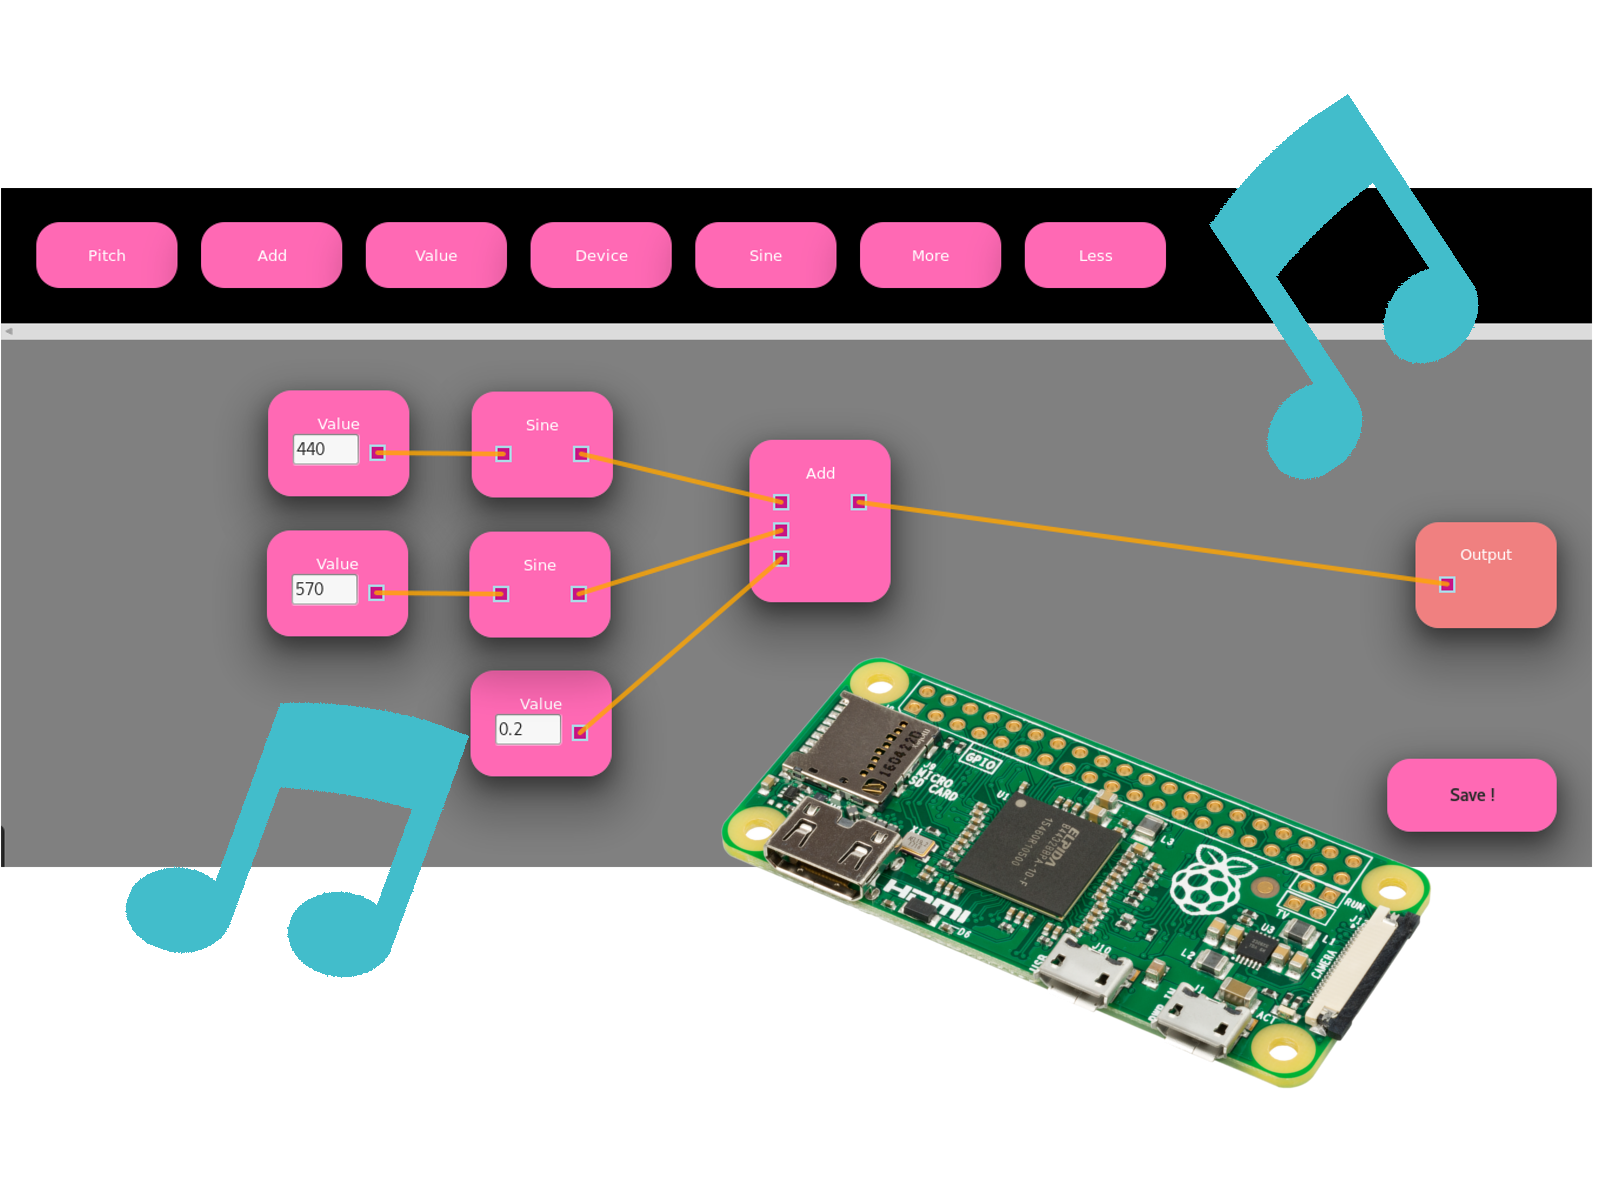
\includegraphics[height=10cm]{presentation_image}
		
		{\Large\itshape Estelle FIKET\\Thomas POTIER\\Nour BOULAHCEN\par}
		\vfill
		encadré par\par
		Mr. Bernigole
		
		\vfill
		
		{\large \today\par}
	\end{titlepage}
	\tableofcontents
	\newpage
	\section{Présentation}
	\paragraph{}
	Dans l'optique de produire un projet intéressant pour l'épreuve de baccalauréat de spécialité ISN, nous avons pensé qu'un projet sur le son était l'idée la plus pertinente quand au programme. Nous avons donc imaginer un système qui permettrait de générer du son en fonction de paramètres physiques tels que l'accélération, la distance ou tout ce qui peut être numérisé.
	\paragraph{}
	En effet, le traitement du son est un domaine qui nous plaisait à tous et nous avons aussi aimer travailler sur le développent Web durant l'année. Nous avons décider de mêler ces domaines dans notre projet. De plus, notre idée ne semblait pas être déjà existante ou tout du moins très peu connue.
	\paragraph{}
	C'est ainsi que nous nous sommes lancés dans "\textit{The Music Swagger}". Nous avons penser à un système qui permettrait de générer du son à partir de données précises, la configuration et les données physiques. Les données physiques seraient récupérées par un petit module de faible taille et la configuration se ferait via une interface Web. 
	
	\section{L'idée}
	Nous avons privilégier l'ergonomie qui permet à un utilisateur non expérimenté de pourvoir simplement utiliser le projet grâce à un fonctionnement "Plug\&Play" et une interface web simpliste.
	
	L'idée du projet est de produire un système permettant grace à des capteurs physiques (tels que gyroscope, mètres ultrasons, ou encore photodiodes), de créer et faire varier des sons afin de générer un son. Nous avons opter pour un système de liaison par wi-fi, et des "devices" à base de Raspberry Pi Zero W pour la portabilité et le prix. Une interface Web sera mise en place afin de pouvoir configurer le comportement de façon simple et sans besoin d'application particulière. Nous avons choisis d'utiliser Python3 pour la plupart des parties pour sa simplicité, sa portabilité ainsi que la richesse de ses modules. L'interface Web est composée de PHP pour l'interaction avec la base de donnée et l'HTML, JS et CSS pour la mise en forme et les interactions avec l'utilisateur (notamment avec le système de "Nodes" en "drag\&drop").
	\subsection{Les différentes parties}
	\subsubsection{Le "brain"}
	C'est une partie simple mais c'est la plus centrale du projet, qui organise les services et gère le programme du "server".
	\subsubsection{Les "devices"}
	C'est la partie englobant tout les capteurs. Elle communique avec le "brain" grâce à un "communicator" (interface de transfert de donnée par réseau (wifi/ethernet)).
	\subsubsection{Le "server"}
	C'est la partie qui permet de générer le son, la réelle partie qui met en forme et concrétise le projet. Elle a un accès à la base de donnée du "configurator" pour se contrôler
	\subsubsection{Le "configurator"}
	C'est l'interface Web basé sur un serveur apache, indépendante du reste du projet par son language (différent de python). Elle communique ses données grâce à une base de donnée. 
	\section{La mise en place}
	\subsection{Répartition}
	Thomas s'est chargé de la partie "device" et "communicator", car il avait déjà des connaissances sur le fonctionnement d'un réseau. Estelle et Nour se sont occupés de la partie "configurator", car ils ont apprécié les projets Web en classe.
	\section{}
	Nous avons choisis un intervalle de rafraîchissement du serveur à 50ms car il faudrait pour ne pas altérer le son avoir au moins une période de chaque fréquence audible tout en gardant un intervalle faible pour ne pas distinguer à l'oreille les changements de valeur. 50ms semble être un bon compromis car il permet d'aller jusqu'à une période de 50ms (soit une fréquence de 20Hz, minimum de l'oreille humaine) et donc peut jouer sans problème toutes les fréquences audibles.
\end{document}
